%%%%%%%%%%%%%%%%%%%%%%%%%%%%%%%%%%%%%%%%%%%%%%%%%%%%%%%%%%%%%%%%%%%%%%%%%%%%%%%%%%%%%%%%%%%%%
%% Poster A0 portrait template University of Tübingen
%
% created by Ekaterina Kohler (ekaterina.kohler@googlemail.com)
% 2022/03/07: completely revised by Chris Nill (chris.nill@student.uni-tuebingen.de)
%
%%%%%%%%%%%%%%%%%%%%%%%%%%%%%%%%%%%%%%%%%%%%%%%%%%%%%%%%%%%%%%%%%%%%%%%%%%%%%%%%%%%%%%%%%%%%%

\documentclass[a0,plainsections]{sciposter}
\usepackage{posterA0} % is located in the same folder as this file and contains all packages and settings

%% your personal packages
%%%%%%%%%%%%%%%%%%%%%%%%%%%%%%%%%%%%%%%%%%%%%%%%%%%%%%%%%%%%%%%%%%%%%%%%%%%%%%%%%%%%%%%%%%%%%
\usepackage{acro}

%% Abbreviations
\DeclareAcronym{vdw}{
short = VdW,
long = Van der Waals
}

%% your personal macros
%%%%%%%%%%%%%%%%%%%%%%%%%%%%%%%%%%%%%%%%%%%%%%%%%%%%%%%%%%%%%%%%%%%%%%%%%%%%%%%%%%%%%%%%%%%%%
\renewcommand{\i}{\mathrm{i}} % imaginary unit
\newcommand{\e}{\mathrm{e}} % Euler-number
\newcommand{\ut}[2]{\underbrace{#1}_{\substack{\text{#2}}}}% Curly bracket description in formula
\newcommand{\ot}[2]{\overbrace{#1}^{\substack{\text{#2}}}}


%%%%%%%%%%%%%%%%%%%%%%%%%%%%%%%%%%%%%%%%%%%%%%%%%%%%%%%%%%%%%%%%%%%%%%%%%%%%%%%%%%%%%%%%%%%%%
%%%%%%%%%%%%------PLEASE FILL IN------%%%%%%%%%%%%%%%%%%%%%%%%%%%%%%%%%%%%%%%%%%%%%%%%%%%%%%%
%%%%%%%%%%%%%%%%%%%%%%%%%%%%%%%%%%%%%%%%%%%%%%%%%%%%%%%%%%%%%%%%%%%%%%%%%%%%%%%%%%%%%%%%%%%%%
\newcommand{\fakult}{Faculty of Science}	% Faculty
\newcommand{\fbname}{Institute for Theoretical Physics\\}
\newcommand{\depart}{Theoretical Atomic Physics and Synthetic Quantum Systems}	% Department or name of the institute
\newcommand{\titel}{Collective decay in a dissipative Rydberg-gas}	%Poster title
\newcommand{\authors}{Chris Nill, Federico Carollo and Igor Lesanovsky}
\newcommand{\authorsAddress}{Institut für Theoretische Physik, Universität Tübingen, Auf der Morgenstelle 14, 72076 Tübingen, Germany}
\newcommand{\presentationDate}{15. Mar. 2022}

\newcommand{\bibPath}{./sources.bib}
%%%%%%%%%%%%%%%%%%%%%%%%%%%%%%%%%%%%%%%%%%%%%%%%%%%%%%%%%%%%%%%%%%%%%%%%%%%%%%%%%%%%%%%%%%%%%

\begin{document}
\maketitle	%Creates header and headings
\vspace*{-20pt}
{\color{rot}{\rule{\textwidth}{4pt}}}

%Enter the structure of the poster. Here 2 columns.
\begin{multicols}{2}

	\addtocounter{figure}{-1}
	\begin{figure}
		\begin{minipage}[t]{0.5\textwidth}
			\section{Rydberg atoms}
			\begin{itemize}
				\item highly excited atoms with high quantum number $n$
				\item energy spectrum similar to hydrogen atom
				\item long lifetime and large radial extension
				      % \item interaction via dipole-dipole $\propto n^4/R^3$
				\item \ac{vdw}-interaction between atoms with distance $R$ scales with $n^{11}/R^6$ \cite{Sibalic2018,Jahangiri2019}
				\item[\textcolor{rot}{$\rightarrow$}]\textcolor{rot}{the excited state of an atom gets shifted upwards by excited neighbours}
			\end{itemize}
		\end{minipage}
		\hfill
		\begin{minipage}[t]{0.48\textwidth}
			\addtocounter{figure}{-1}
			\begin{figure}
				\vspace*{-175pt} % Spaltenausrichtung minipages
				\captionsetup{type=figure}
				\includesvg[width=\textwidth]{./images/Rydberg-Potential.svg}
				\caption{\textbf{An atom in the Rydberg potential of its neighbours.} The excited state gets shifted upwards by the potential of the neighbours.}
				\label{fig:RydbergPotential}
			\end{figure}

		\end{minipage}%
	\end{figure}

	\vspace*{-10pt}
	\addtocounter{figure}{-2}
	\begin{figure}
		\section{The system}
		\begin{figure}
			\centering
			\captionsetup{type=figure}
			\vspace*{-40pt} % weißen rand des bildes entfernen
			\includesvg[width=0.8\linewidth]{./images/IMG_generalSetting.svg}
			\caption{\textbf{Schematic description of the considered model of a strongly interacting Rydberg gas with nearest neighbour interaction.}\\ Lattice distance $R$, energy spacing $\omega_a$, Rabi frequency $\Omega$, detuning $\Delta$, single atom decay rate $\gamma$}
		\end{figure}

		\begin{figure}
			\begin{AutoMultiColItemize}
				\item 1D chain of strongly interacting Rydberg atoms \\(modelled as 2-level systems $\ket{g},\ket{s}$)
				\item driven by a laser with Rabi frequency $\Omega$
				\item assume cyclic boundary conditions
				\item lattice spacing $R$ much larger than transition wavelength $\rightarrow$ neglecting collective decay processes \cite{nott61187}
				\item \ac{vdw} potential treated as nearest-neighbour interaction \cite{Olmos2009,Ates2012}
			\end{AutoMultiColItemize}
		\end{figure}
	\end{figure}

	\begin{figure}
		\section{Local approach: Master equation}
		\begin{AutoMultiColEnumerate}
			\item derive the master equation without Rydberg interaction and laser, see (eq. \ref{eq:HamiltonMitBad}, black only)
			\item add interaction afterwards \cite{nott61187} and obtain \eqref{eq:masterSingle}
			\item[\textcolor{rot}{$\rightarrow$}] \textit{jump operators $L_k=\sigma_k$} act on single atom only
			\item[\textcolor{rot}{$\rightarrow$}] \textcolor{rot}{Is this really justified in a Rydberg gas with strong interactions?}
		\end{AutoMultiColEnumerate}
		\vspace*{-2\abovedisplayskip} %remove formula whitespace
		\begin{alignat}{3}
			\dot\rho=-\i\comm{H}{\rho}+ \gamma \sum_k \bigg(& \sigma_k & \rho \sigma_k^\dagger & - \frac{1}{2}\acomm{\sigma_k^\dagger \sigma_k}{\rho}\bigg) & \label{eq:masterSingle} \\[-1.5em]\nonumber
			                                  & \uparrow &                       &                                                      &                         \\[-0.5em]\nonumber
			                                  & L_k      &                       &                                                      &
		\end{alignat}
		\vspace*{-3\belowdisplayskip} %remove formula whitespace
	\end{figure}

	\addtocounter{figure}{-2}
	\begin{figure}
		\section{Consequence of strong interactions}
		\begin{itemize}
			\item Consider strong interactions between nearest neighbours $\Rightarrow$ 3 distinguishable configurations
			\item define an orthonormal set of projectors $P^\xi_k$ for each neighbour configuration $\xi$ of an atom $k$
		\end{itemize}
		\textit{\textcolor{rot}{In principle, the configurations can be distinguished by their different frequencies of emission!}}
		\begin{figure}
			%\vspace*{-75pt} %rand von bild entfernen
			\centering
			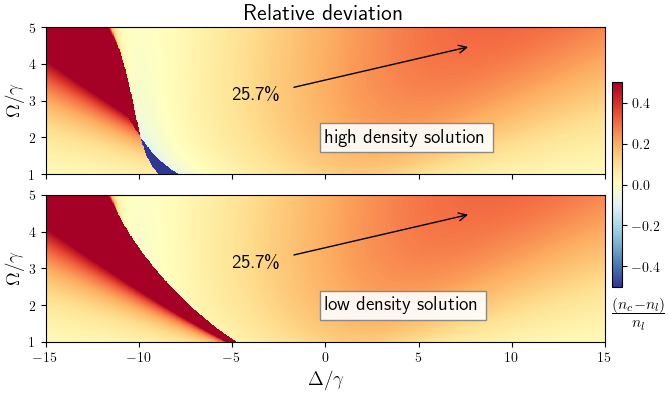
\includegraphics[width=0.5\textwidth]{./images/DemoPlot.png}
			%\vspace*{-120pt} %rand von bild entfernen
		\end{figure}
	\end{figure}

	\addtocounter{figure}{-2}
	\begin{figure}
		\section{Collective approach: Master equation}
		Derive the master equation in presence of nearest neighbour interactions \cite{Gonzalez2017}.\\
		We proceed analogously to \cite{Breuer_2007,lidar2020lecture,Schaller2015} and obtain \eqref{eq:masterCollective}.
		\begin{align}
			H & =
			\ot{
			\ut{\omega_a\sum_k{n_k}}{bare atom energy}
			\textcolor{rot}{+\ut{V \sum_k{n_kn_{k+1}}}{Rydberg interaction}}
			+\ut{\sum_q{\omega_q a_{q}^\dagger a_q}}{bath energy}
			}{$H_0$}
			+\ut{\sum_{q,k}{g_{qk}(a_q \e^{\i \vb{q \cdot r}_k}+a_{q}^\dagger\e^{-\i \vb{q \cdot r}_k})\sigma_k^x}}{system-bath interaction}
			\label{eq:HamiltonMitBad}
		\end{align}
	\end{figure}
	\addtocounter{figure}{-2}
	\begin{figure}
		\begin{AutoMultiColEnumerate}
			\item transform into interaction picture via unitary\\ $U=\text{exp}(\i H_0 t)$
			\item apply Born-Markov approximation
			\item apply rotating-wave approximation
			\item assume large Rydberg interaction $V/\gamma\gg 1$
			\item define the configuration dependent decay rate $\Gamma^\xi$ with dipole matrix element $\vb{d_{gs}}=\mel**{g}{e\vb{r}}{s}$
			\begin{equation}
				\Gamma^\xi =
				\frac{\abs{\vb{d_{gs}}}^2}{3 \pi \hbar \epsilon_0 c^3}
				(\omega_a+\xi V)^3
				\label{eq:GammaXi}
			\end{equation}
		\end{AutoMultiColEnumerate}
	\end{figure}
	\begin{shaded}
		\textbf{Collective master equation}
		\begin{equation}
			\dot\rho_\text{int}  = \mathlarger{\mathlarger{\sum}}_{\xi=\left\{ 0,1,2 \right\}}
			\Gamma^\xi
			\sum_k \ut{\sigma_k P_k^\xi}{$L_k^\xi$} \rho\ P_k^\xi \sigma_k^\dagger
			+ \acomm{ \sigma_k P_k^\xi \sigma_k^\dagger}{\rho}
			\label{eq:masterCollective}
		\end{equation}
		\begin{AutoMultiColItemize}
			\renewcommand\labelitemi{\textcolor{rot}{$\rightarrow$}}
			\item jump operators change to collective jump operators $L_k^\xi=\sigma_k P_k^\xi$
			$\Rightarrow$ dissipation is configuration dependent
			%\item each configuration $\xi$ decays with specific rate $\Gamma^\xi$
		\end{AutoMultiColItemize}
	\end{shaded}


	\addtocounter{figure}{-1}
	\begin{figure}
		\begin{minipage}{\textwidth}
			\section{Driven dissipative Rydberg gas within collective approach}
			\begin{AutoMultiColItemize}
				\item drive system with a laser with Rabi frequency $\Omega$ and detuning $\Delta$
				\item study the excitation density $\expval{n}$ in the steady stationary state
				%\item use equation of motion formalism \cite{Schaller2015}
				\item apply mean-field approximation $\expval{n \sigma_x}=\expval{n}\expval{\sigma_x}$ and homogenize atoms$\expval{n_k}=\expval{n_{k'}}$ \cite{PhysRevLett.101.250601}
			\end{AutoMultiColItemize}
			\begin{itemize}
				\renewcommand\labelitemi{\textcolor{rot}{$\rightarrow$}}
				\item \textcolor{rot}{for the collective approach we obtain an additional summand $4\expval{n}$ (in red)} in the system of equations \eqref{eq:mean-field}, which comes from the entry of the neighbouring atoms
				\item depending on chosen parameters $\Omega$ and $\Delta$ either 1 or 3 solutions result
				\item either 1 or 2 are stable $\rightarrow$ study only those
			\end{itemize}
			\begin{minipage}[c][][t]{0.54\textwidth}
				\begin{shaded}
					\textbf{System of equations}
					\begin{alignat}{7}%[leftmargin=0pt]
						 & \expval{\dot{n}}        &  & =  & \Omega \expval{\sigma_y} & - \gamma \expval{n}                                                           &  &                                   &  & \nonumber             \\
						 & \expval{\dot{\sigma}_x} &  & =- & \Delta \expval{\sigma_y} & -\frac{\gamma}{2}(\mathbin{\textcolor{rot}{4\expval{n}}}+1) \expval{\sigma_x} &  & -2 V \expval{n} \expval{\sigma_y} &  & \label{eq:mean-field} \\
						 & \expval{\dot{\sigma}_y} &  & =- & \Delta \expval{\sigma_x} & -\frac{\gamma}{2}(\mathbin{\textcolor{rot}{4\expval{n}}}+1)\expval{\sigma_y}  &  & +2 V \expval{n} \expval{\sigma_x} &  & \nonumber             \\ %[-1.5em]
						 &                         &  &    &                          & -2\Omega (2\expval{n} -1)                                                     &  &                                   &  & \nonumber
					\end{alignat}
				\end{shaded}
			\end{minipage}
			\hfill
			\begin{minipage}[c][][t]{0.44\textwidth}
				\captionsetup{type=figure}
				\centering
				\vspace*{-10pt} % Remove white border on top of plot
				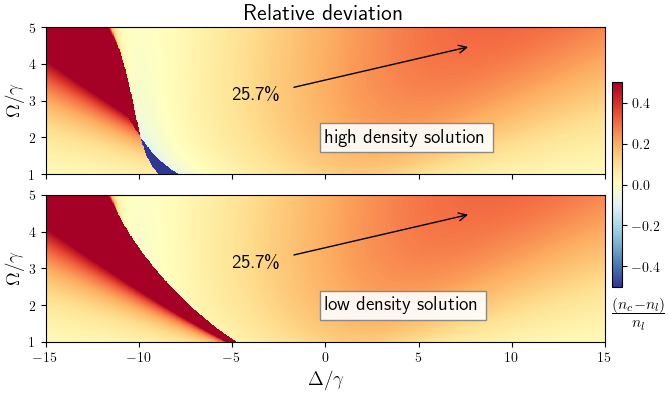
\includegraphics[width=\textwidth]{./images/DemoPlot.png}
				\vspace*{-60pt} % Remove white border under plot
				\caption{
					\textbf{Number of solutions with the collective approach $(c)$, the local approach $(l)$.}
					We set $V=10\gamma$. We observe a shift in phase boundaries and critical points.}
				\label{fig:NofSols}
			\end{minipage}
		\end{minipage}
	\end{figure}

	\addtocounter{figure}{-2}
	\begin{figure}
		\begin{minipage}[t]{0.5\textwidth}
			\begin{figure}
				\captionsetup{type=figure}
				\centering
				\vspace*{-60pt}
				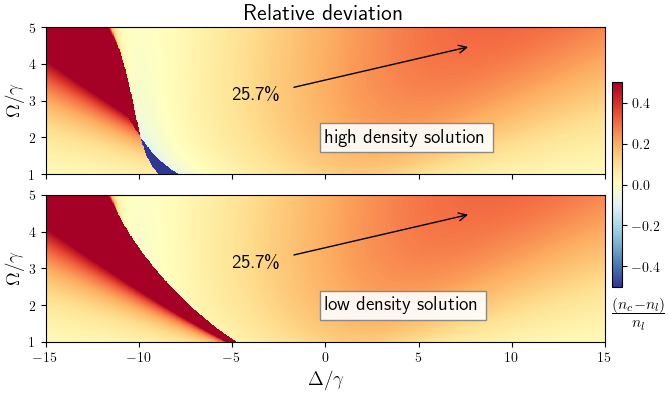
\includegraphics[width=\textwidth]{./images/DemoPlot.png}
				%\vspace*{-60pt} % weißen Rand vom Plot entfernen
				\caption{\textbf{Excitation density phase diagrams for collective and local approach.} $V=10\gamma$.
					The low density solution corresponds to the smallest of the 3 solutions, the high density to the largest. We observe a shift in the phase boundaries for both solutions.
				}
				\label{fig:AbsSols}
			\end{figure}
		\end{minipage}
		\hfill
		\begin{minipage}[t]{0.47\textwidth}
			\captionsetup{type=figure}
			\centering
			\vspace*{-16pt}
			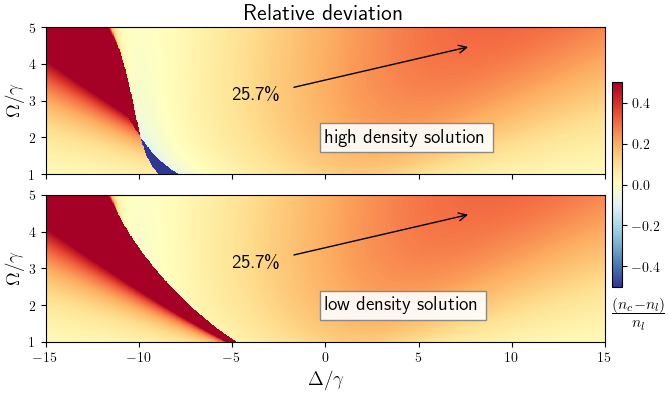
\includegraphics[width=\textwidth]{./images/DemoPlot.png}
			\vspace*{-40pt} % weißen Rand vom Plot entfernen
			\caption{\textbf{Relative deviation of the phase diagrams} with collective vs. the local approach. We set $V=10\gamma$.	The low density solution corresponds to the smallest of the 3 solutions, the high density to the largest. In the area of the transitions from \figref{fig:NofSols} we find a high relative deviation here.}
			\label{fig:DiffofSols}
		\end{minipage}
	\end{figure}

	\addtocounter{figure}{-2}
	\begin{figure}[h]
		\begin{minipage}{0.55\textwidth}
			\section*{Relative deviation for finite number of particles}
			\begin{itemize}
				\item for particle numbers $N<6$, we use the method of exact diagonalization
				      % by means of the Choi-Jamilkowski formalism
				      \cite{Schaller2015}. For $N\geq6$, we use the \glqq continuous-time Monte Carlo\grqq\ algorithm from \cite{Plenio1998}.
				\item simulations are done with Python framework QuTiP \cite{qutip1,qutip2}.
				\item[\textcolor{rot}{$\rightarrow$}] in \figref{fig:numericResults} similar parameter regimes for differences compared to the mean-field calculations can be identified
				\item[\textcolor{rot}{$\rightarrow$}] clear differences for $\Delta/ \gamma<-5$: Excitation density is higher for the collective approach
				\item periodic effects in Monte Carlo calculations are most likely due to residual oscillations of the equilibrium state after finite simulation time
			\end{itemize}
		\end{minipage}
		\hfill
		\begin{minipage}{0.4\textwidth}
			\begin{figure}
				\captionsetup{type=figure}
				\vspace*{-50pt} % remove whitespace on top of plot
				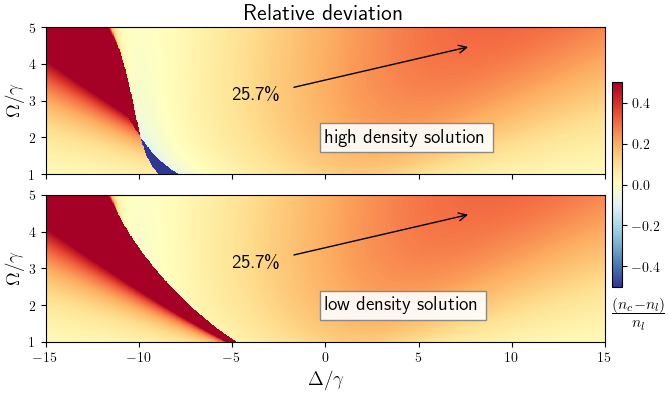
\includegraphics[width=\linewidth]{./images/DemoPlot.png}
				\vspace*{-60pt}
				\caption{\textbf{Relative deviation of phase diagrams with finite number of particles $N$} at $V=10\gamma$. Normalized by the number of particles.}
				\label{fig:numericResults}
			\end{figure}
		\end{minipage}
	\end{figure}

	\section{Conclusion}
	\begin{AutoMultiColItemize}
		\renewcommand\labelitemi{\textcolor{rot}{$\rightarrow$}}
		\item The dissipation of a strongly interacting Rydberg gas changes due to its interaction.
		\item Frequency and rate of spontaneous decay of an atom depends on configuration of neighbouring atoms.
		\item Shift in phase boundaries and critical points occurs.
		\item Excitation density $\expval{n}$ in mean-field approximation shows a significant deviation compared to the local approach for certain parameter choice.
		\item With finite particle number, we observe a relative deviation up to $\SI{120}{\percent}$, which grows with system size.
	\end{AutoMultiColItemize}
\end{multicols}

\vspace*{-10pt}
\textcolor{rot}{\rule{\textwidth}{4pt}}
\setlength{\columnseprule}{0pt}
\begin{multicols}{2}
	\vspace*{-70pt}
	\printbibliography[heading=customBibTitle]
	\vspace*{-10pt}

	\section*{Contacts}
	{\small
		Chris Nill\\
		chris.nill@student.uni-tuebingen.de\\
		Auf der Morgenstelle~14\\
		72076~Tübingen, Germany
	}
\end{multicols}
\end{document}
